
    \chapter{External Climate Variables prediction}

    \section{chapter}{Inndoor Climate Model}

    
    \section{Inner temperature Modelling}

    En este sección solo consideraremos la temperatura interior $x_{T}$ como variable de estado.
    
    \begin{gather}
        Q = Q_{ext} + Q_{heater} + Q_{radiation}
    \end{gather}
    
    Capacidad calorífica 
    \begin{gather}
        C_d = \lim_{\Delta T \to \infty}\frac{Q}{\Delta T}
    \end{gather}
    
    La transferencia de la temperatura de un medio es muy proceso muy conocido estudidas en el siglo XVII. Esta variación de la temperatura puede provenir de tres tipos de fuentes. Estas son mediante convección, conducción y radiación. Las fuentes puede afectar al estado del sistema mediante:
    \begin{enumerate}
        \item \textbf{Heat Sources}: Añadiendo fuentes de energía. Debido a la conservación de la energía.
        \begin{enumerate}
            \item Conduction Sources: Transmisión de calor por contacto sin transferencia de materia.
            \item Convection Sources: Transmisión de calor por contato con transferencia de materia. En nuestro caso el Heater $u_T$ y la temperatura exterior $f_T$.
            \item Radiation Sources: Transmisión de calor por ondas electromagneticas. En nuestro caso la radiación exterior $f_r$.
        \end{enumerate}
        \item \textbf{Perturbation}: Alteración en la menera en la que se conduce la temperatura:
        \begin{enumerate}
            \item Conduction Perturbation: Transmisión de calor por contacto sin transferencia de materia.
            \item Convection Perturbation: $u_w$: Windows.
            \item Radiation Perturbation:  $u_r$:             Shade screens
        \end{enumerate}
    \end{enumerate}
    De esta manera, podemos entender la naturaleza de nuestas fuentes controladas y no controladas. Además de ciertas restricciones que deben cumplir la variación de las fuentes. Por ejemplo, la variación de las perturbaciones nunca debe generar energía sino favorecer o mitigar su transmición. 
    
    Por el contrario las fuentes de calor podrían afectar la manera en la que el sistema intercambia  temperatura, es decir que la capacidad calorífica de los disitnos elementos pueda depender de la temperatura, sin embargo obviaremos este efecto por simplificidad
    
    %%%%%%%%%%%%%%%%%%%%%%%%%%%%%%%
    \subsection{Modelos }
    
    \subsubsection{Cooling Newton law with external sources}
    
    \begin{model}{Cooling Newton law with external sources}{}\label{model:CoolNewton}
    Consider the following variables: 
    \begin{center}
        \begin{tabular}{|c|c|c|c|c|}
            \hline
            \textbf{Type} & \textbf{Dim} &\textbf{Name} & \textbf{Notation} & \textbf{Units} \\
                \hline
                \multirow{1}{*}{States}  & $\bm{x} \in \mathbb{R}$& Inner Temperature & $x_{T}$ & $K$ \\
                \hline
                \hline
                \multirow{2}{*}{Sources} & \multirow{2}{*}{$\bm{f} \in \mathbb{R}^2$} & Exterior Temperature & $f_{T}$ & $K$ \\
                & & Exterior Radiation & $f_{r}$ & $W/m^2$ \\
                \hline
                \hline
                \multirow{1}{*}{Controls} & $\bm{u} \in \mathbb{R}$ & Heater         & $u_{T}$ & $W$ \\
                \hline
        \end{tabular}    
    \end{center}
        Given a exterior temperature $f_{T}$, the inner temperature of greenhouse $x_{T}$ can be determined by following ordinaly differential equation:  
        \begin{gather}\label{eq:CoolNewton_plus_sources}
            \frac{dx_{T}(t)}{dt} = -\underbrace{c_d[x_{T}(t) - f_{T}(t)]}_{\text{Newton law}} + 
            3.6e3  \Bigg[ 
                \underbrace{ \Bigg( \frac{u_{T}(t)}{c_H} \Bigg) }_{\text{Heater Term}} + 
                \underbrace{ \Bigg( \frac{f_{r}(t)}{ c_R } \Bigg) }_{\text{Radiation Term}} \Bigg]
        \end{gather}
        Parámetros a estimar 
        \begin{enumerate}
            \item $c_d( h^{-1})$: Coeficiente de difusión del invernadero.
            \item $c_H(JK^{-1})$: Capacidad calorífica del invernadero debido a las calderas.
            \item $c_R(JK^{-1}m^{-2})$: Capacidad calorífica del invernadero por unidad de superficie debido a la radiación.
        \end{enumerate}
    \end{model}
    
    
    
    Ajustamos este modelo con la Trayectoria \ref{traj:noheater}. Suponiendo que esta trayectoria tiene una señal de heater $u_T(t) = 0$ , podemos simplificar la formula \eqref{eq:CoolNewton_plus_sources}:
    
    \begin{gather}
        \frac{dx_{T}(t)}{dt} = -c_d[x_{T}(t) - f_{T}(t)] + 
        3.6e3     \Bigg( \frac{f_{r}(t)}{ c_R } \Bigg)  
    \end{gather}
     
    Entonces para $t \in \{t_1,t_2,\dots,t_T\}$
    \begin{gather}
    \frac{dx_{T}(t)}{dt} = \begin{bmatrix}
        -(x_T(t) - f_T(t)) & 3.6e3 f_r(t) 
    \end{bmatrix} \begin{bmatrix}
        c_d \\ (1/c_R)
    \end{bmatrix}
    \end{gather}
    
    
    De manera que tenemos podemos formular una ecuación matricial
    
    \begin{gather}
        \underbrace{
        \begin{bmatrix}
            \frac{dx_{T}}{dt}(t_1) \\
            \frac{dx_{T}}{dt}(t_2) \\
            \frac{dx_{T}}{dt}(t_3) \\
            \dots
        \end{bmatrix}}_{d\bm{X}} = 
        \underbrace{\begin{bmatrix}
            -(x_T(t_1) - f_T(t_1)) & 3.6e3 f_r(t_1)  \\
            -(x_T(t_2) - f_T(t_2)) & 3.6e3 f_r(t_2)  \\
            -(x_T(t_3) - f_T(t_3)) & 3.6e3 f_r(t_3)  \\
            \dots
        \end{bmatrix}}_{G} \begin{bmatrix}
            c_d \\ (1/c_R)
        \end{bmatrix}
        \end{gather}
    
    Entonces 
    \begin{gather}
        \begin{bmatrix}
            c_d \\ (1/c_R)
        \end{bmatrix} =  \bm{G}^{-1}d\bm{X}
    \end{gather}
    
    Donde $\bm{G}^{-1}$ es la pseudo-inversa de Penrose. 
    \newline
    
    Hemos obtenido $c_d(h^{-1}) = 0.0054$, $ c_R(JK^{-1}m^{-2}) = 1.5519e+04$. Obteniendo $RMSE \approx 4 ^\circ C$. Además, suponiendo que el modelo obtenido es capaz de reproducir el comportamiento del invernadero podemos obtener una señal de heater asociada a la Trayectoria \ref{traj:heater}.
    
    
    \begin{figure}
        \centering
        % T01_CLIMA_2020_02_04_A003
        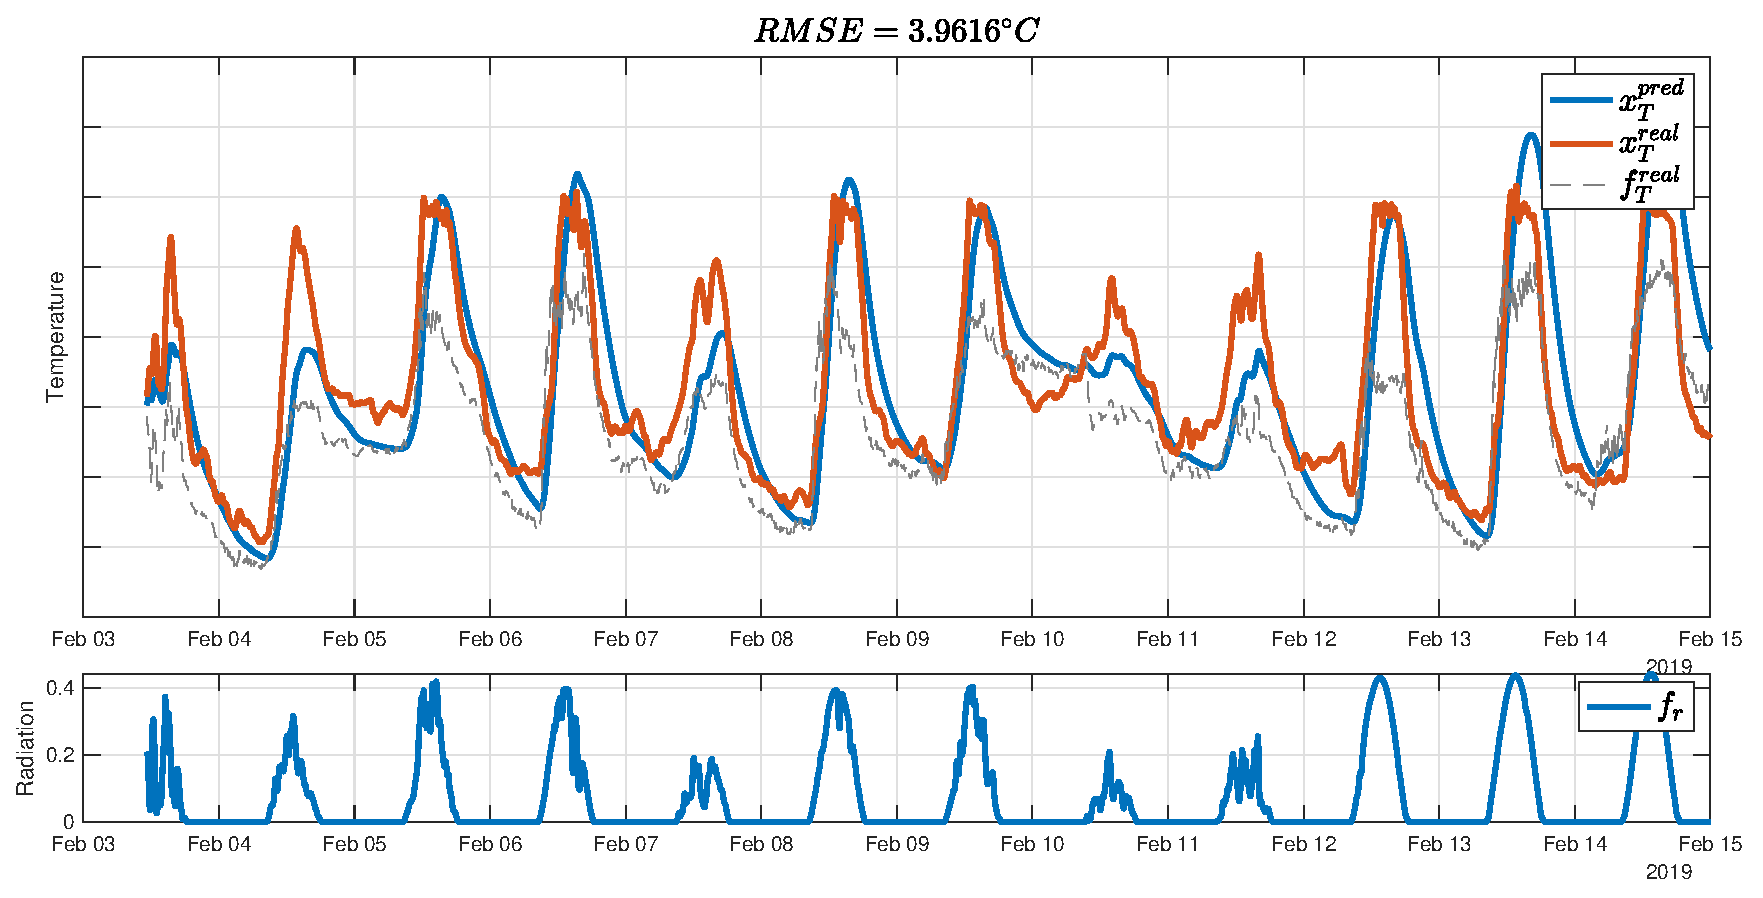
\includegraphics[scale=0.5]{img/model-2.1.1.eps}
    \end{figure}
    
    
    \subsubsection{Newton Law \& external sources with variable convection diffusion}
    Presentamos una manera huerística del efecto de las ventanas en la temperatura interior.
    
    
    
    \begin{model}{Newton Law \& external sources with variable convection diffusion}{}
    
    \begin{gather}
        \frac{dx_{T}(t)}{dt} =  
        -\underbrace{c_d(u_{w}(t))}_{\text{Windows}\atop\text{dependence}}[x_{T}(t) - f_{T}(t)] +
        %
        \Bigg[ \frac{3.6 \times 10^{3}}{c_H} \Bigg] u_{T}(t)+ 
        \Bigg[ \frac{3.6 \times 10^{3}}{ c_R } \Bigg] f_r(t)
    \end{gather}
    Donde:
    \begin{gather}
        c_d(u_w) =  c_d^{min} + (c_d^{max} - c_d^{min})\frac{u_{w}}{100}
    \end{gather}
    
    Parámetros a estimar
    \begin{enumerate}
        \item $c_d^{min}( h^{-1})$: Coeficiente de difusión del invernadero debido a las calderas con las ventanas cerradas.
        \item $c_d^{max}( h^{-1})$: Coeficiente de difusión del invernadero debido a las calderas con las ventanas abiertas. 
        \item $c_R(JK^{-1}m^{-2})$: Capacidad calorífica del invernadero por unidad de superficie debido a la radiación.
    \end{enumerate}
    \end{model}
    
    \begin{model}{Modelo híbrido}{}
    \begin{gather}
        \frac{dx_{T}(t)}{dt} = c_{\omega_d}(.)[x_{T}(t) - f_{T}(t)] + c_{\omega_f}(.) 
    \end{gather}
    Donde los parámetros de difusión y el término de fuentes son aproximados por percpetrones multicapa.
    \begin{gather}
        c_{\omega_d} = c_{\omega_d}(u_w,f_H) \\
        c_{\omega_f} =  c_{\omega_f}(u_T,u_r,f_r)
    \end{gather}
    \end{model}
    
    
    \begin{model}{NARX}{}
    Consideramos las siguiente variables:
    \begin{center}
        \begin{tabular}{|c|c|c|c|c|}
            \hline
            \textbf{Type} & \textbf{Set} &\textbf{Name} & \textbf{Notation} & \textbf{Units} \\
                \hline
                \multirow{3}{*}{States} & 
                \multirow{3}{*}{$\bm{x} \in \mathbb{R}^3$}&
                    Inner Temperature & $x_{T}$ & $K$ \\
                & & Inner Radiation & $x_{r}$ & $W/m^2$ \\
                & & Inner Relative Humidity & $x_{h}$ & $\%$\\
                \hline
                \hline
                \multirow{4}{*}{Sources } &
                \multirow{4}{*}{$\bm{f} \in \mathbb{R}^4$} &
                    Exterior Temperature & $f_{T}$ & $K$ \\
                & & Exterior Radiation & $f_{r}$ & $W/m^2$ \\
                & & Exterior Relative Humidity & $f_{h}$ & $\%$\\
                & & Wind Velocity & $f_w$ & $Km/h$  \\
                \hline
                \hline
                \multirow{3}{*}{Controls} &
                \multirow{3}{*}{$\bm{u} \in \mathbb{R}^3$} &
                    Heater         & $u_{T}$ & $W$ \\
                & & Windows        & $u_{w}$ & $\%$ \\
                & & Shade screens  & $u_{r}$ & $\%$\\
                    \hline
        \end{tabular}  
    \end{center}
    
    Let $\Delta t$, we can define a NARX model of oder 1:
    \begin{gather}
        \bm{x}(t+\Delta t) = c_{\omega_d} \Big[ \bm{x}(t),\bm{u}(t),\bm{f}(t),\bm{x}(t-\Delta t),\bm{u}(t-\Delta t),\bm{f}(t-\Delta t)  \Big]
    \end{gather}
    
    \end{model}
    
    
    
    \begin{model}{ANN}{}
        Consideramos las siguiente variables:
        \begin{center}
            \begin{tabular}{|c|c|c|c|c|}
                \hline
                \textbf{Type} & \textbf{Set} &\textbf{Name} & \textbf{Notation} & \textbf{Units} \\
                    \hline
                    \multirow{3}{*}{States} & 
                    \multirow{3}{*}{$\bm{x} \in \mathbb{R}^3$}&
                        Inner Temperature & $x_{T}$ & $K$ \\
                    & & Inner Radiation & $x_{r}$ & $W/m^2$ \\
                    & & Inner Relative Humidity & $x_{h}$ & $\%$\\
                    \hline
                    \hline
                    \multirow{4}{*}{Sources } &
                    \multirow{4}{*}{$\bm{f} \in \mathbb{R}^4$} &
                        Exterior Temperature & $f_{T}$ & $K$ \\
                    & & Exterior Radiation & $f_{r}$ & $W/m^2$ \\
                    & & Exterior Relative Humidity & $f_{h}$ & $\%$\\
                    & & Wind Velocity & $f_w$ & $Km/h$  \\
                    \hline
                    \hline
                    \multirow{3}{*}{Controls} &
                    \multirow{3}{*}{$\bm{u} \in \mathbb{R}^3$} &
                        Heater         & $u_{T}$ & $W$ \\
                    & & Windows        & $u_{w}$ & $\%$ \\
                    & & Shade screens  & $u_{r}$ & $\%$\\
                        \hline
            \end{tabular}  
        \end{center}
        
        Let $\Delta t$, we can define a NARX model of oder 1:
        \begin{gather}
            \bm{x}(t+\Delta t) = c_{\omega_d} \big(\bm{u}(t),\bm{f}(t) \big)
        \end{gather}
        
        \end{model}
    